\documentclass{article}
\usepackage{graphicx}
\usepackage{amsmath}
\usepackage{array}
\usepackage[font=small, labelfont={sf,bf}, margin=1cm]{caption}
\usepackage{tabularx}
\usepackage{amssymb}
\usepackage{multirow}



\date{Due:Nov 21 Edit: \today}
\title{PHYS 225 HW 11}
\author{James Liu}

\begin{document}
\maketitle
\begin{itemize}
    \item [1.]
    \begin{itemize}
        \item [a)]
        \begin{align*}
            p_\pi&=\sqrt{E^2-m^2}\\
            &=990.15 \times 10^6 \text{ eV}
        \end{align*}
        in the lab frame:
        \begin{align*}
            \mathbf{p}_1&=(E_1,p_1,0,0)\\
            \mathbf{p}_2&=(E_2,p_2,0,0)\\
            \mathbf{p}_3&=(p_3,p_3,0,0)\\
            \mathbf{p}_1&=\mathbf{p}_2+\mathbf{p}_3\\
            &\left\{\begin{matrix}
                990.15 \times 10^6 =p_2+p_3\\
                10^9 =E_2+p_3
            \end{matrix}\right.\\
            E_2&=\sqrt{m_{\mu}^2+p_2^2}\\
            &=\sqrt{(106\times 10^6)^2+p_2^2}\\
            &\left\{\begin{matrix}
                p_2=564.43 \text{ MeV}\\
                p_3=424.72 \text{ MeV}
            \end{matrix}\right.\\
            E_\nu &= p_3 = 424.72 \text{ MeV}\\
        \end{align*}
        the the direction is also colinear with the pion's momentum direction.
        \newpage
        \item [b)]\
        \begin{figure}[h]
            \centering
            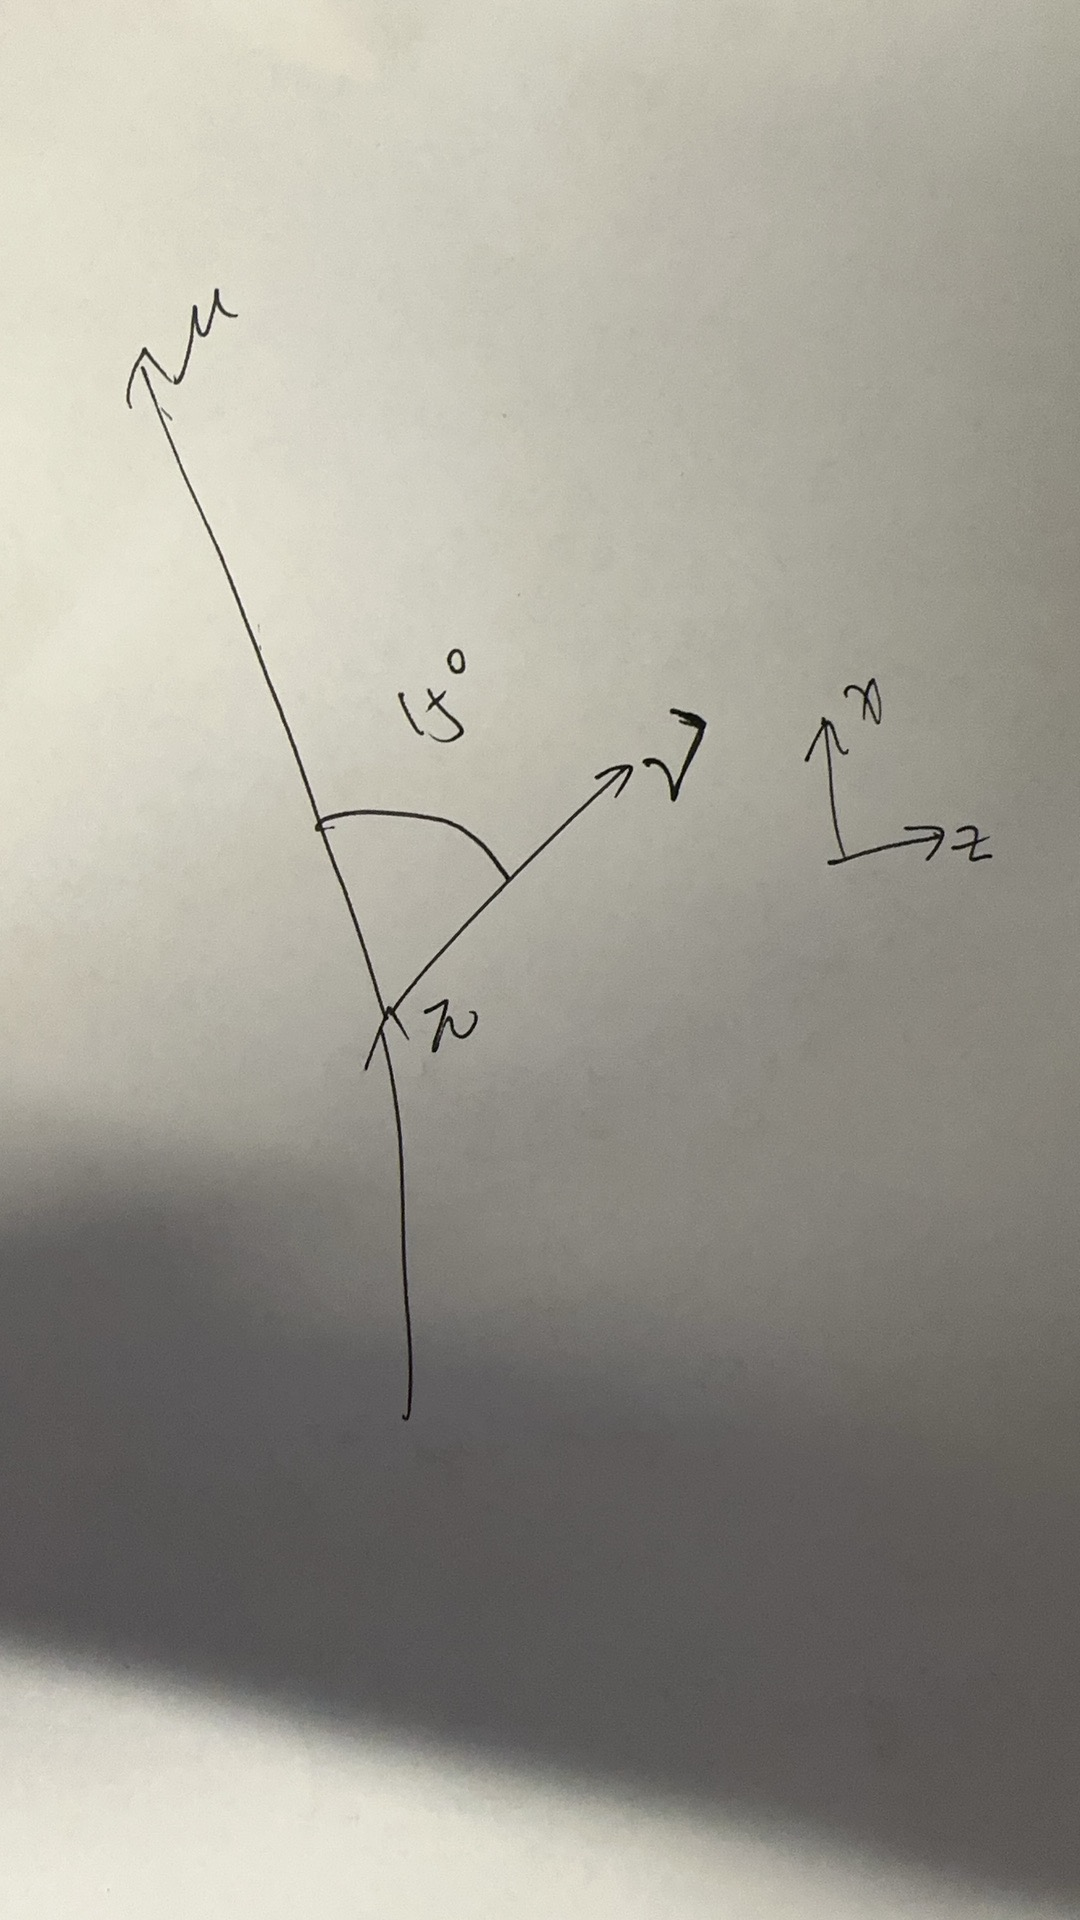
\includegraphics[scale=0.08]{figure/phys225_hw11_fig1_alt.jpeg}
        \end{figure}
        \begin{align*}
            \\
            \mathbf{p}_1&=(E_1,p_1,0,0)\quad (\pi)\\
            \mathbf{p}_2&=(E_2,p_{2x},p_{2y},p_{2z})\quad (\mu)\\
            \mathbf{p}_3&=(||p||,p_{3x},p_{3y},p_{3z}) \quad (\nu)\\
            \mathbf{p}_1&=\mathbf{p}_2+\mathbf{p}_3\\
            ||p_3||&=E_1-E_2\\
            &=100 \text { MeV}\\
            ||p_2||&=\sqrt{E_2^2-m^2}\\
            &= \sqrt{900^2-106^2}\\
            &=893.736 \text{ MeV}\\
        \end{align*}
        Set \(p_{2y}=p_{3y}=0\), then:
        \begin{align*}
            \left\{\begin{matrix}
                p_{2x}+p_{3x}=990.15\\
                p_{2z}+p_{3z}=0\\
                ||p_2||=893.736\\
                ||p_3||=100
            \end{matrix}\right.
        \end{align*}
        Solving this will give:
        \begin{align*}
            \overrightarrow{p_\mu}&=(893.38,0,-25.2117)\\
            \overrightarrow{p_\nu}&=(96.7697,0,25.2117)\\
            \cos(\theta)&= \frac{\overrightarrow{p_\nu}\cdot\overrightarrow{p_\mu}}{||\overrightarrow{p_\mu}|| \ ||\overrightarrow{p_\nu}||}\\
            &=0.962199\\
            \theta &=15.8041 ^\circ
        \end{align*}
    \end{itemize}
    \newpage
    \item [2.] 
    \begin{align*}
        p_1 &=\frac{E}{c} = p_{2x}+p_{3x}\\
        &=p_2\cos(\theta)+p_3\cos(\theta)\\
        p_{2y}\sin(\theta)-p_{3y}\sin(\theta)&=0\\
        p_2&=p_3\\
        \frac{E}{c}&=2p_{rst}\cos(\theta)\\
        p_{rst}c&=\frac{E}{\cos(\theta)}\\
        E'_{m}&=\sqrt{p^2c^2+m^2c^4}\\
        E+E_m&=E'_m+E_{rst}\\
        E+E_m&=\sqrt{E_{rst}^2+m^2c^4}+E_{rst}\\
        ((E+mc^2)^2-E_{rst})^2&=E_{rst}^2+m^2c^4\\
        E_{rst}&=\frac{E(E+2mc^2)}{2(E+mc^2)}\\
        \cos(\theta)&=\frac{E}{2E_{rst}}=\frac{E+mc^2}{E+2mc^2}\\
        E\rightarrow 0, &\ \cos(\theta)\rightarrow \frac{1}{2},\ \theta \rightarrow 60^\circ
    \end{align*}
\end{itemize}
\end{document}